\begin{figure}
  \centering
  \captionsetup[subfigure]{aboveskip=2pt, belowskip=3pt}

  \begin{subfigure}{0.44\textwidth}
    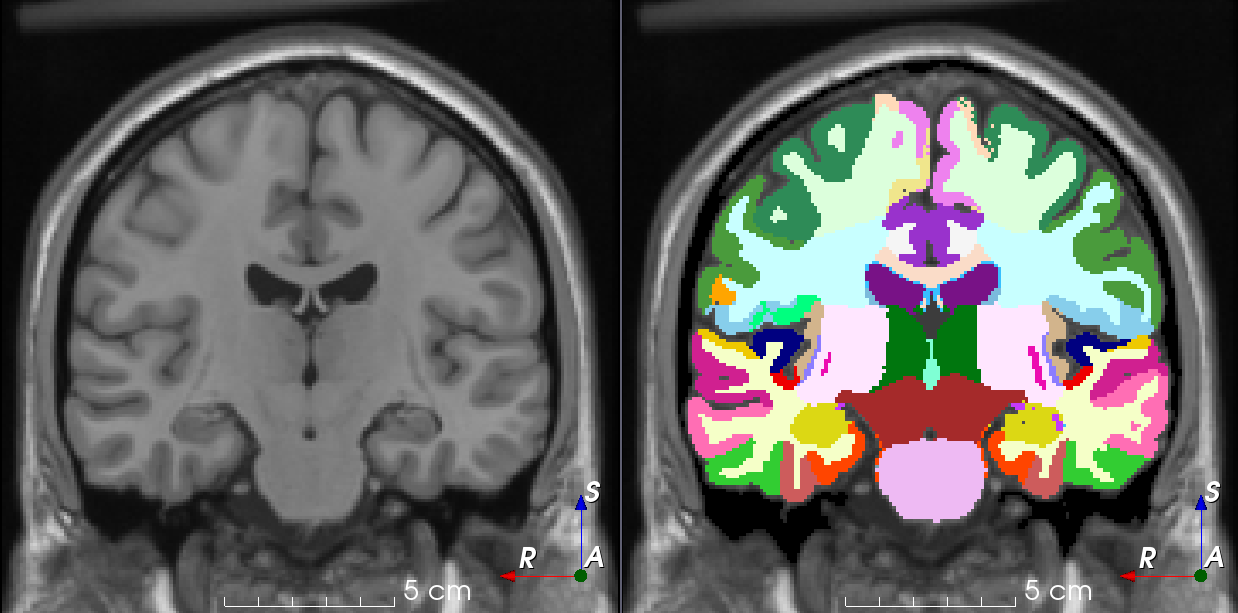
\includegraphics[width=0.98\linewidth]{colin27_t1_tal_lin_mri}
    \caption{Original image and segmentation}
    \label{fig:original}
  \end{subfigure}%
  \hspace{2em}%
  \begin{subfigure}{0.44\textwidth}
    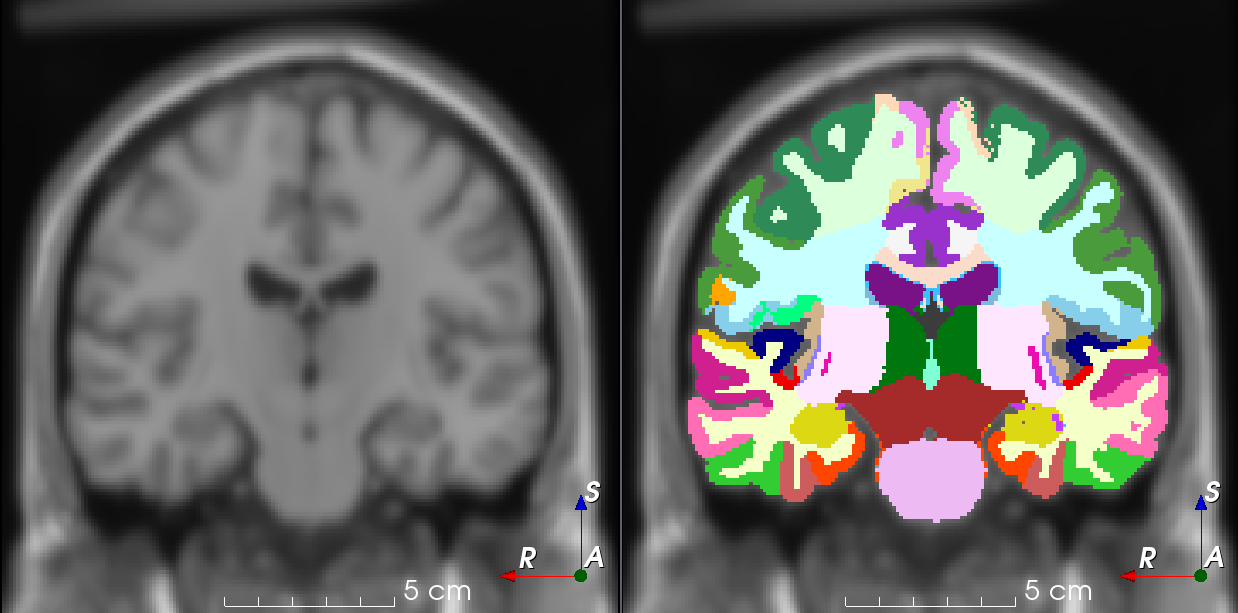
\includegraphics[width=0.98\linewidth]{0_RandomBlur_mri}
    \caption{Random blur}
    \label{fig:rblur}
  \end{subfigure}

  \begin{subfigure}{0.44\textwidth}
    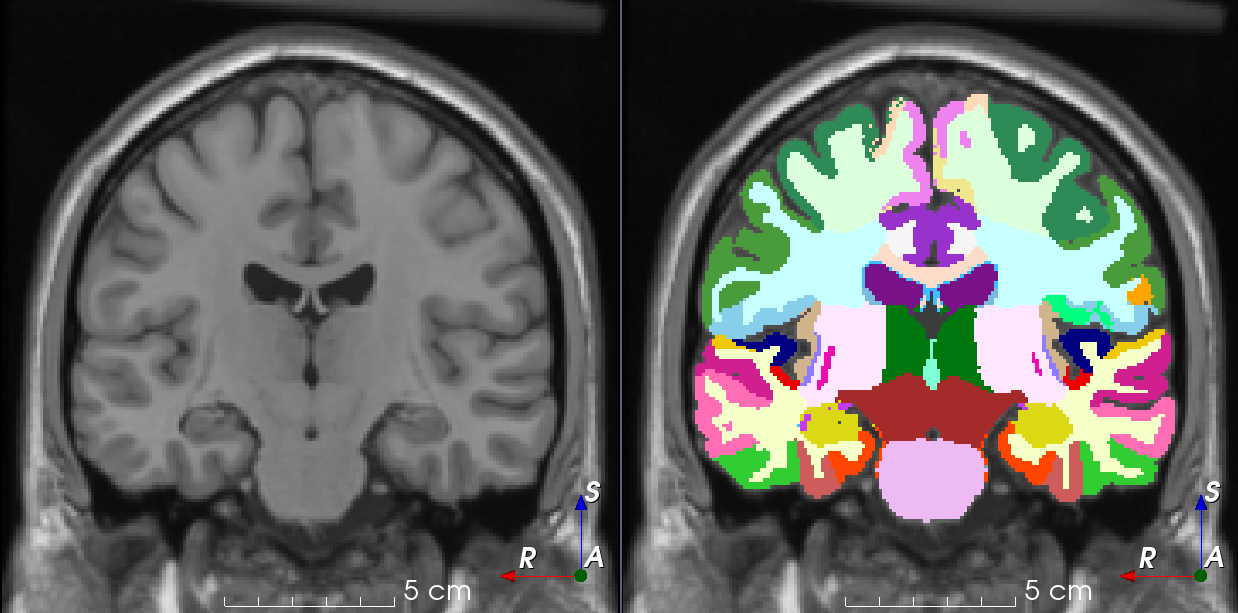
\includegraphics[width=0.98\linewidth]{1_RandomFlip_mri}
    \caption{Random flip}
    \label{fig:rflip}
  \end{subfigure}%
  \hspace{2em}%
  \begin{subfigure}{0.44\textwidth}
    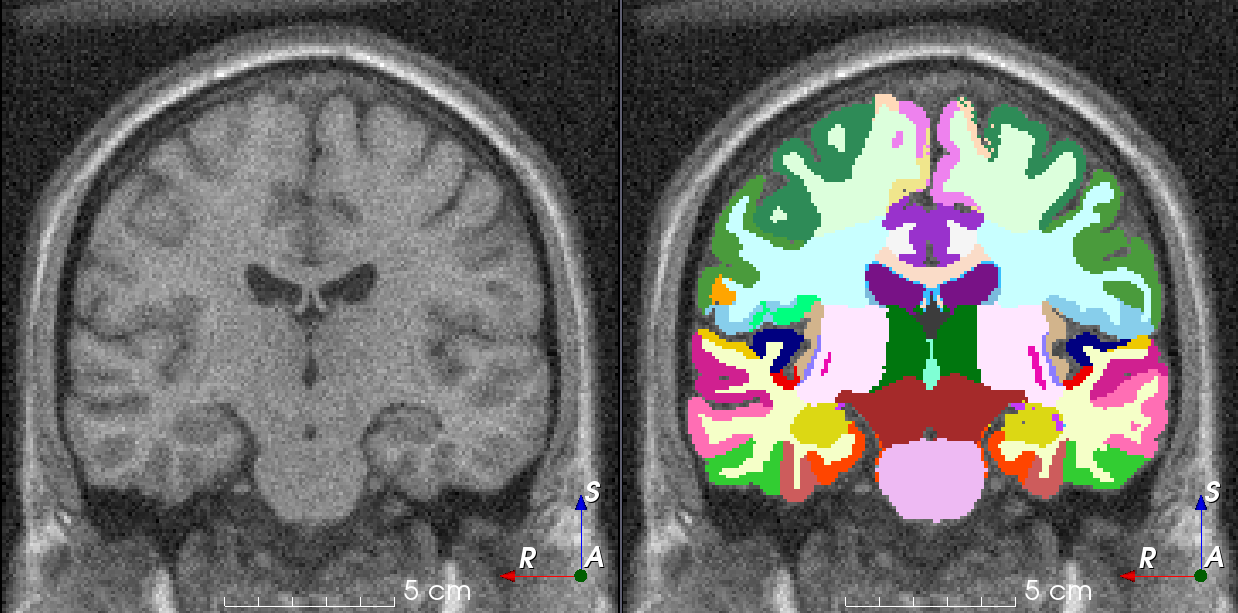
\includegraphics[width=0.98\linewidth]{2_Compose_mri}
    \caption{Random noise}
    \label{fig:rnoise}
  \end{subfigure}

  \begin{subfigure}{0.44\textwidth}
    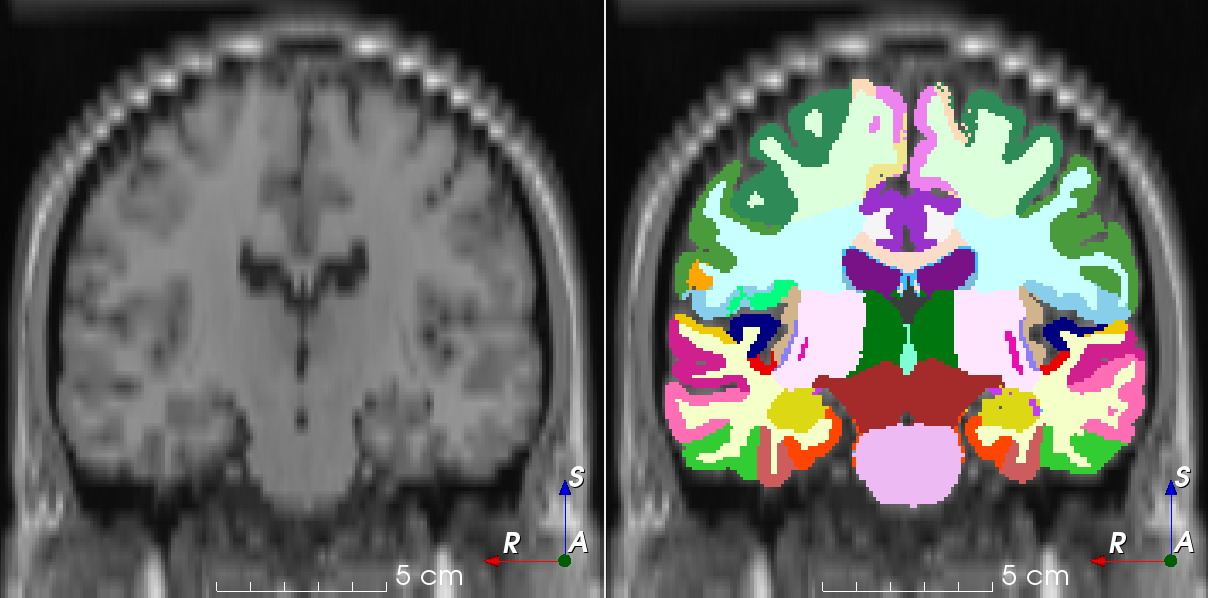
\includegraphics[width=0.98\linewidth]{0_RandomAnisotropy_mri}
    \caption{Random anisotropy}
    \label{fig:raffine}
  \end{subfigure}%
  \hspace{2em}%
  \begin{subfigure}{0.44\textwidth}
    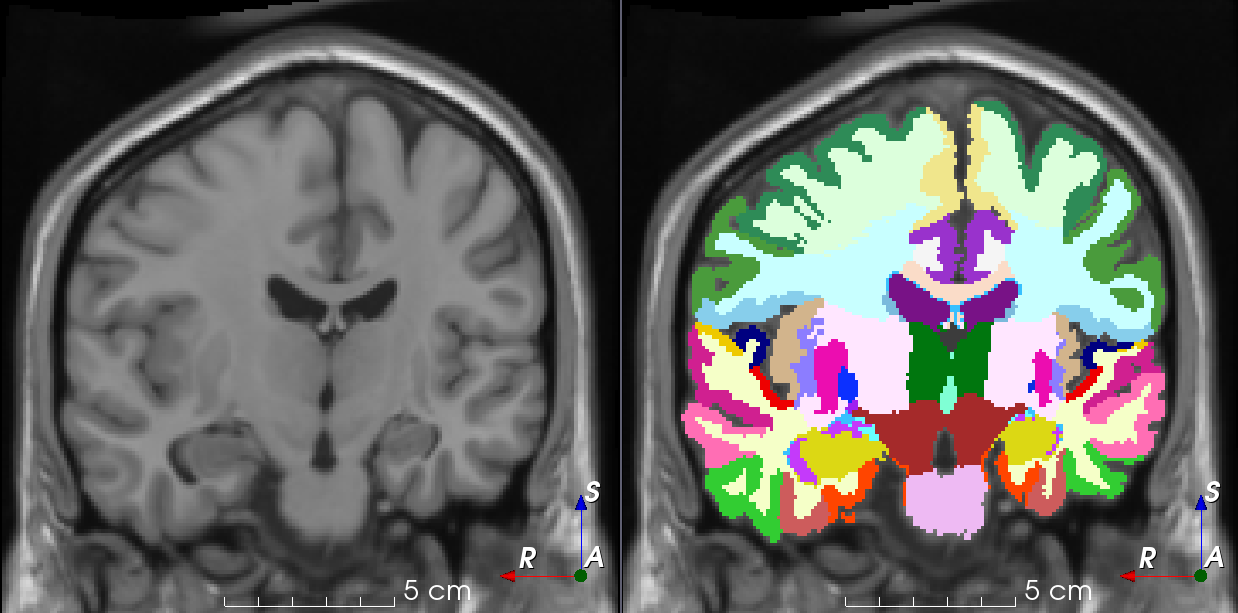
\includegraphics[width=0.98\linewidth]{4_RandomElasticDeformation_mri}
    \caption{Random elastic transformation}
    \label{fig:relastic}
  \end{subfigure}

  \begin{subfigure}{0.44\textwidth}
    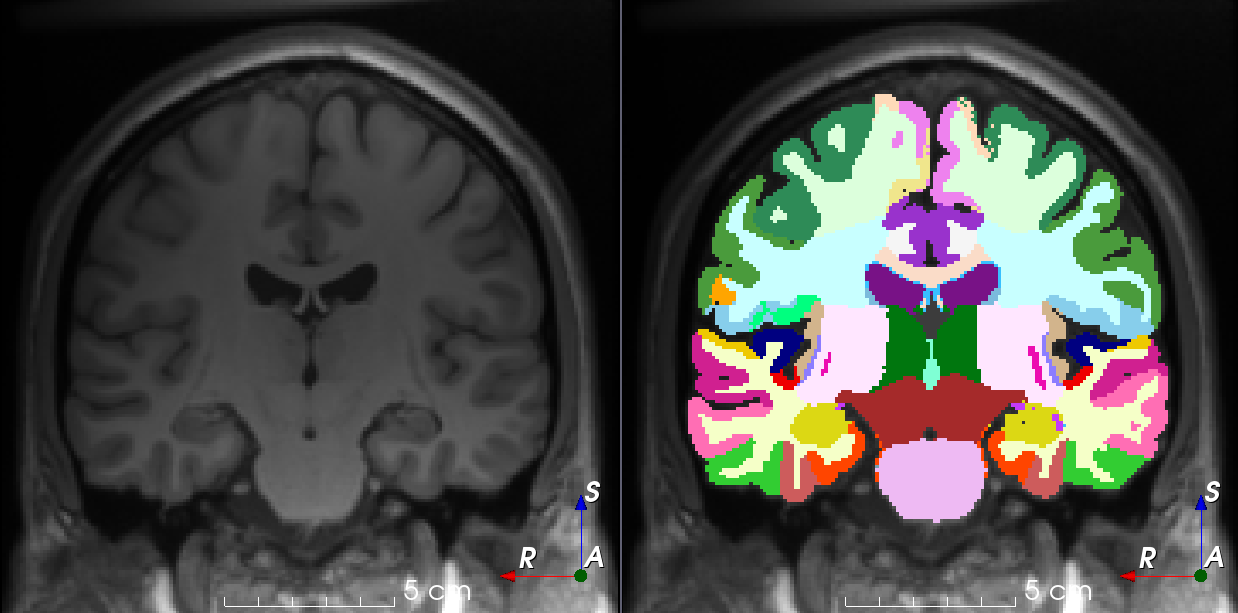
\includegraphics[width=0.98\linewidth]{5_RandomBiasField_mri}
    \caption{Random bias field artifact}
    \label{fig:rbias}
  \end{subfigure}%
  \hspace{2em}%
  \begin{subfigure}{0.44\textwidth}
    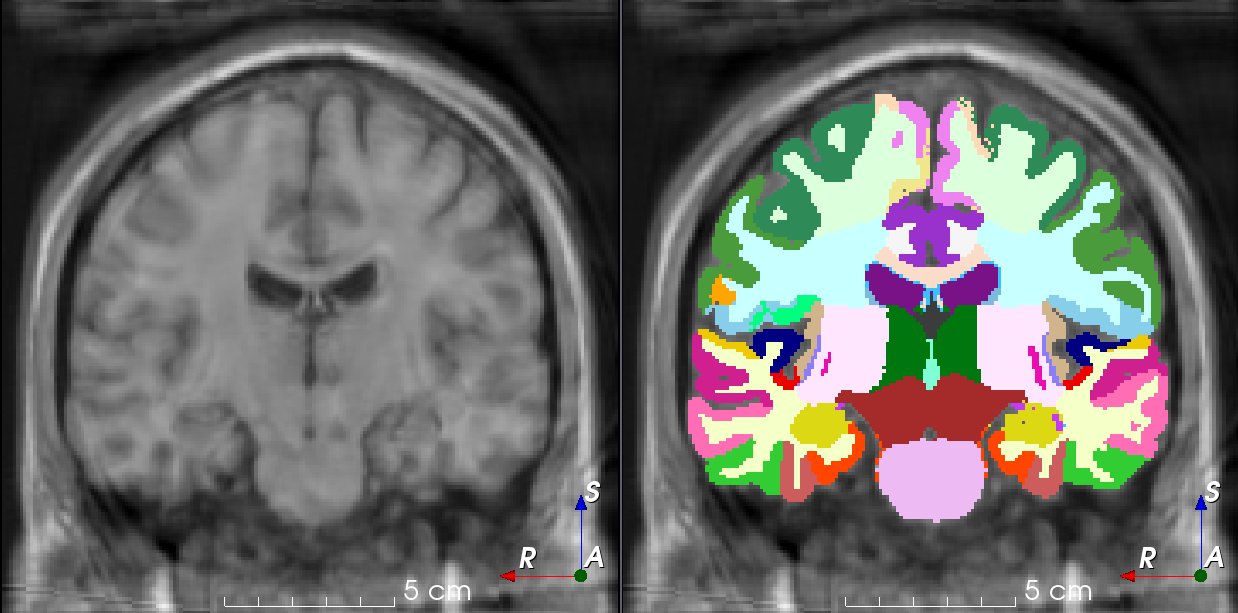
\includegraphics[width=0.98\linewidth]{6_RandomMotion_mri}
    \caption{Random motion artifact}
    \label{fig:rmotion}
  \end{subfigure}

  \begin{subfigure}{0.44\textwidth}
    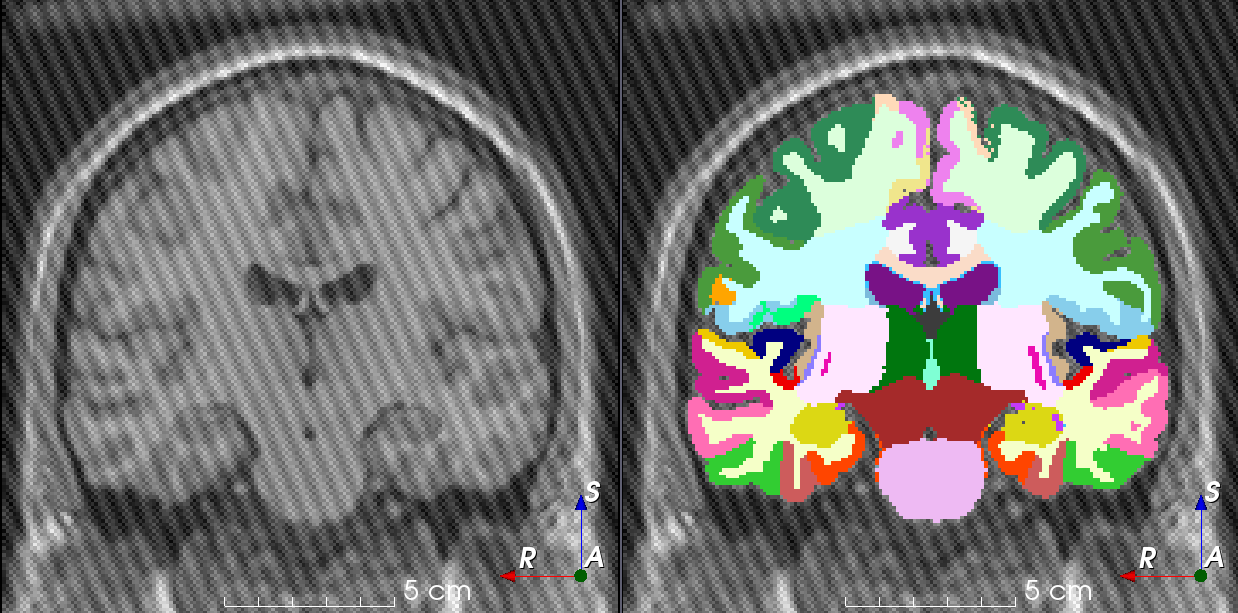
\includegraphics[width=0.98\linewidth]{7_RandomSpike_mri}
    \caption{Random spike artifact}
    \label{fig:rspike}
  \end{subfigure}%
  \hspace{2em}%
  \begin{subfigure}{0.44\textwidth}
    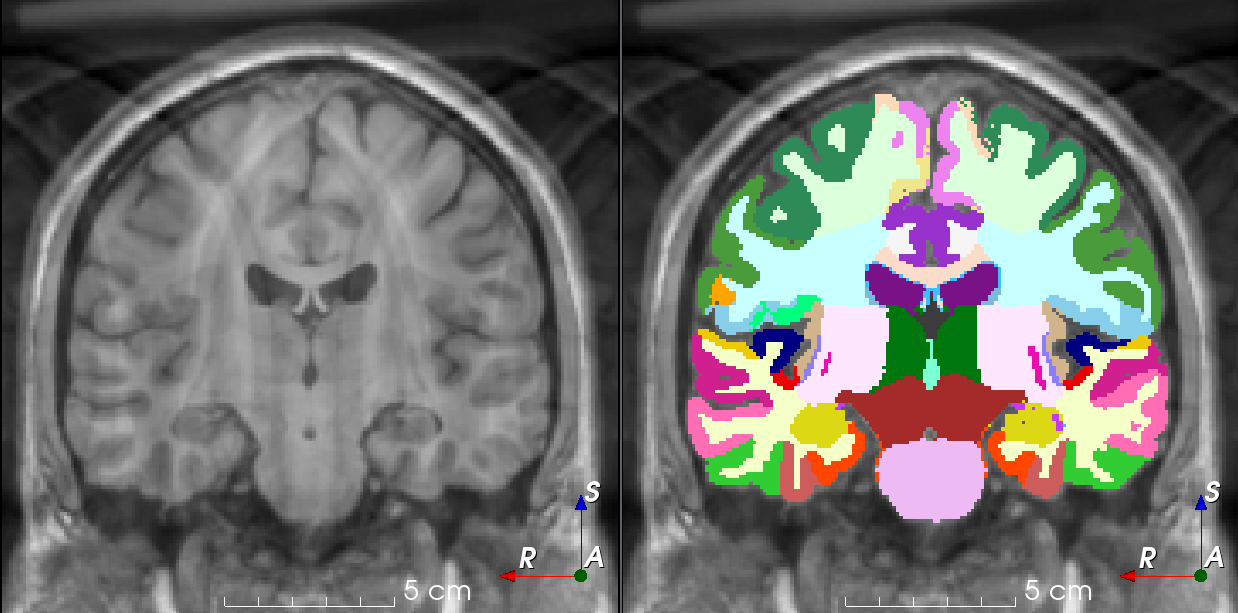
\includegraphics[width=0.98\linewidth]{8_RandomGhosting_mri}
    \caption{Random ghosting artifact}
    \label{fig:rghost}
  \end{subfigure}

  \caption[A selection of data augmentation techniques available in TorchIO \torchioversion]{
    A selection of data augmentation techniques available in TorchIO \torchioversion.
    Each example is presented as a pair of images composed of the transformed image and a corresponding transformed label map.
    Note that all screenshots are from a 2D coronal slice of the transformed 3D images.
    The \ac{MRI} corresponds to the \ac{MNI} Colin 27 average brain \cite{holmes_enhancement_1998}, which can be downloaded using \texttt{torchio.datasets.Colin27}.
    Label maps were generated using an automated brain parcellation algorithm \cite{cardoso_geodesic_2015}.
  }
  \label{fig:augmentations}
\end{figure}

% \acreset{mni}  % we want to describe it in the text as well
